\chapter{Wprowadzenie technologiczne}
\label{cha:wprowadzenieTechnologiczne}

%---------------------------------------------------------------------------

\section{DynamoDB}
\label{sec:dynamoDb}


Do aplikacji, które wykorzystują podejście data-driven trzeba wykorzystywać bazy danych, które pozwalają na przechowywanie i zarządzanie dużymi ilościami danych. Takie aplikacje rzadko mają skomplikowany model, zwykle składa się on z niewielu tabel, które zawierają bardzo duże ilości rekordów.

Amazon DynamoDB to system bazodanowy rozproszony pomiędzy wieloma partycjami oferujący wysoką wydajność. Dużym atutem tego systemu jest skalowalność, ponieważ jesteśmy w stanie dodawać nowe maszyny do klastra w trakcie działania systemu. Jest to możliwe, ponieważ każdy wiersz w tabeli ma określoną maszynę na której się znajduje poprzez wyliczenie jego skrótu (ang. hash) algorytmem “Consistent hashing”.  Dane rozłożone na wielu maszynach są szybciej dostępne oraz bezpieczniejsze, ponieważ w całym systemie nie ma pojedynczego punktu, który mógłby spowodować awarię całej bazy danych.


Kluczowe cechy DynamoDB:

\begin{enumerate}
    \item Brak jednoznacznej struktury w tabeli.

Podobnie jak w relacyjnej bazie danych - struktura DynamoDB składa się z tabel, które zawierają rekordy (DynamoDB nie nakłada limitu na liczbę rekordów w tabeli, barierą jest jedynie pamięć fizyczna). W odróżnieniu od systemów relacyjnych - rekordy w DynamoDB nie posiadają ustalonej struktury. Jedyną rzeczą jaką musi posiadać dany rekord jest Partition Key.

    \item Rozproszenie danych.

DynamoDB może przechowywać dane w obrębie jednej tabeli na kilku fizycznych maszynach - jest to możliwe dzięki Partition Key używany jest on jako argument funkcji haszującej, której wynik decyduje na której maszynie znajdzie się rekord. Konsekwencją jest to, że szukając jakichkolwiek danych musimy znać ich Partition Key lub mieć stworzony indeks na innym atrybucie - w przeciwieństwie do klasycznych systemów relacyjych, zapytania wykorzystujące dowolny atrybut jako warunek nie są dozwolone.

    \begin{figure}[H]
    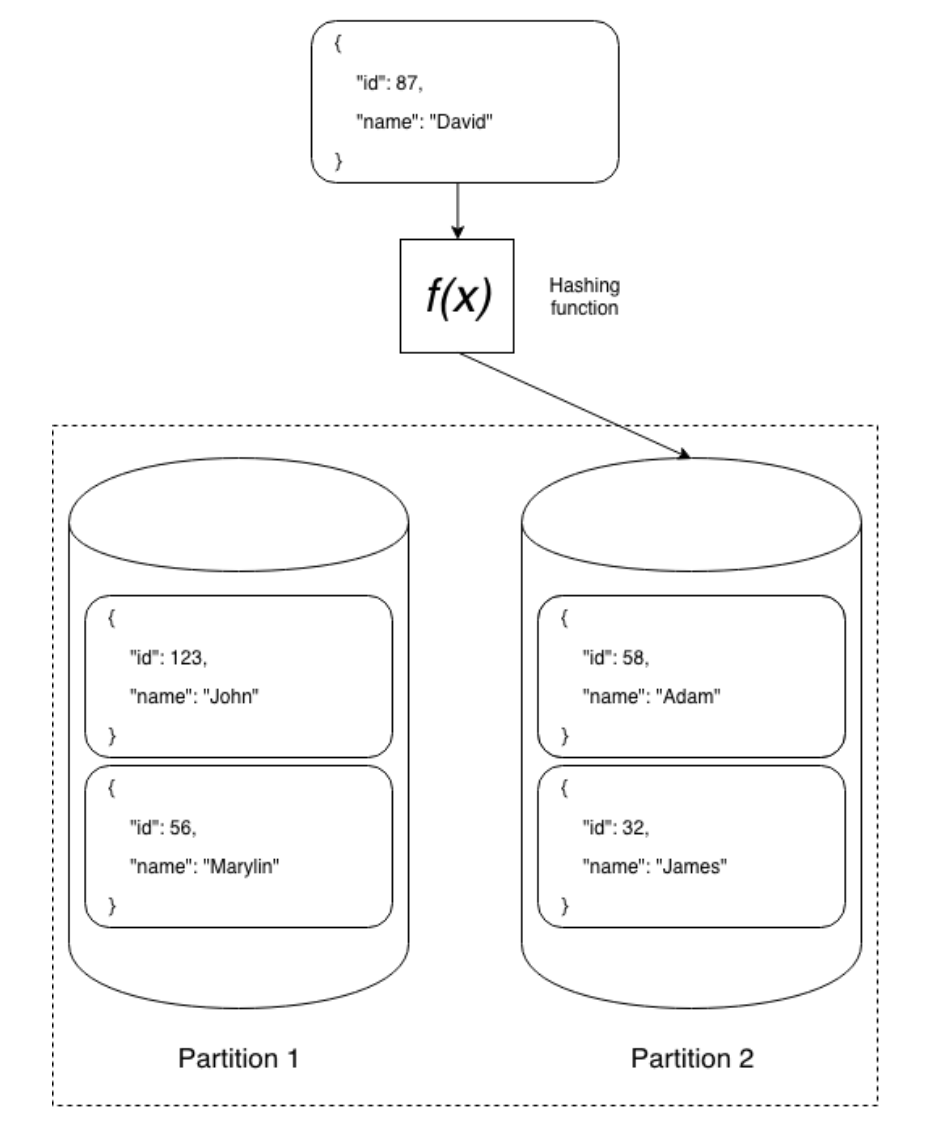
\includegraphics[width=11cm]{dynamo_partitions.png}
    \centering
    \caption{Schemat umieszczania rekordu w DynamoDB}
    \end{figure} 

    \item Eventual/Strong Consistency.

System bazodanowy DynamoDB pozwala nam na działanie w dwóch poziomach konsystencji. Strong consistency pozwala nam na odczytanie najbardziej aktualnych danych znajdujących się w systemie. Ma on jedno ważne wymaganie - wszystkie maszyny w systemie muszą być sprawne (co w systemach rozproszonych nie jest wcale oczywiste). Mamy też drugi poziom bardziej odpowiadający charakterystyce systemów rozproszonych - Eventual consistency. W tym trybie istnieje ryzyko otrzymania nieaktualnych danych - natomiast zapewnione jest, że jeśli powtórzymy zapytanie po pewnym czasie, dane zostaną uaktualnione. Czas ten jest inny dla każdego systemu - zależy on od szybkości replikacji danych.

    \item Skalowalność horyzontalna.

Im więcej danych przechowujemy, tym więcej partycji je przechowuje. Zwiększanie rozmiarów tabeli nie wpływa na wydajność kwerend wykonywanych na nich. 

    \item “No single point of failure”

Dzięki zastosowaniu wielu partycji, z których każda działa niezależnie - system jest częściowo odporny na awarie. Nasze dane nie są przechowywane na jednej maszynie, dzięki czemu nie grozi nam całkowita utrata przechowywanych danych.
\end{enumerate}


\section{Serverless}
\label{sec:serverless}

W ostatnich latach technologie “serverless” zyskały dużą popularność wraz z rozwojem chmur obliczeniowych. Ta technologia jest znana także jako FaaS (function as a service), ponieważ dostawca usług chmurowych zapewnia nam całą infrastrukturę oraz zarządzanie nią, podczas gdy my (jako klienci) musimy dostarczyć tylko funkcję (kod programu), jaka będzie wykonywana podczas zapytania do usługi. Wybrane zalety usług “serverless” to:

\begin{enumerate}
    \item Skalowalność - funkcja  wdrożona w środowisku serverless może w nim przebywać nie generując kosztów jeśli nie jest ona wywoływana. Z drugiej strony, gdy mamy do czynienia z dużym ruchem - infrastruktura wykonująca nasze funkcje jest skalowana horyzontalnie, dzięki czemu infrastruktura nie jest ograniczeniem wydajności aplikacji.
    
    \item Czas potrzebny od napisania kodu do uruchomienia go na serwerze jest dużo mniejszy niż przy użyciu infrastruktury on-premise. Cała konfiguracja oraz zarządzanie środowiskiem jest odpowiedzialnością dostawcy usług chmurowych.
\end{enumerate}

Pomimo zalet trzeba również pamiętać o innych cechach tych usług, które trzeba wziąć po uwagę, gdy planujemy tworzyć aplikację pod kątem działania jako serverless:

\begin{enumerate}
    \item “Cold start” - jest to czas potrzebny na uruchomienie środowiska aplikacji. Jeśli nasza funkcja nie jest wywoływana przez dany czas, jej środowisko zostaje wyłączone, przez co pierwsze wywołanie po takim czasie zajmuje znacznie więcej czasu niż pozostałe. Efekt ten jest zależny od czasu startu oraz pamięci wymaganej przez aplikację, czyli w C# oraz Java będzie on znacznie bardziej uciążliwy niż dla funkcji zaimplementowanych w Python.3

    \item Przetwarzanie długich zapytań - większość dostawców usług “serverless” ma limity czasowe na wykonanie jednego wywołania funkcji. Każdy proces, który zajmie dłużej jest natychmiast zakończony. Aplikacje, posiadające takie cechy potrzebują poważnych zmian w architekturze zanim zostaną przeniesione na usługi “serverless”.
\end{enumerate}
